\section{Introduction}

\andrew{Make sure to tie this into what my contributions are to our class and what they should take away.}

As you enter the Invention Lab, Berkeley's student hackerspace, you quickly notice that learning to work with fabrication machines is hard.
Scorched cardboard sits atop the scrap pile from laser-cut materials that caught fire.
Failed 3D prints line the foyer walls, deformed from thin supports and improper orientations.
Consider what it takes to configure a laser cutter to ``raster'' images onto workpieces:
four different parameters control the depth, speed, and fidelity of the image etched into the material.
Improper values cause the image to appear only faintly, or melt the material (see Figure~\ref{fig:rasters}).

This research pursues a vision for fabrication machines that help users learn how to operate them.
My key insight is that a fabrication machine can be equipped with an active learning algorithm to enable mixed initiative exploration of a parameter space.
I implement this for a laser cutter and a maker rastering images.
My intended contributions are:
\begin{enumerate}
\item A catalog of user problems realizing design intent with laser cutters
\item Application of active learning to discovering an ideal fabrication machine configuration
\item A comparison of mixed initiative parameter exploration with self-led approaches
\end{enumerate}

To understand frequency, severity, and types of errors makers encounter with laser cutters, I will interview a small number of student members of the Invention Lab.

I will implement an active learning algorithm~\cite{settles_active_2010} to guide a machine, with a user's help, to some subjective ideal configuration for rastering an image.
Each configuration will comprise laser power, speed, frequency, and resolution.
The algorithm will suggest configurations and demonstrate them by rastering an image.
The algorithm will collect a user's rating of raster quality.
As the learned model will predict an continuous value, I will draw from past work for actively learning continuous-value models (e.g.~\cite{sugiyama_active_2008}).
% Currently, I suspect that a Gaussian kernel function or a quadratic curve will best express a user's perception of the quality of a configuration in actualizing their design.

\begin{figure}
  \centering
  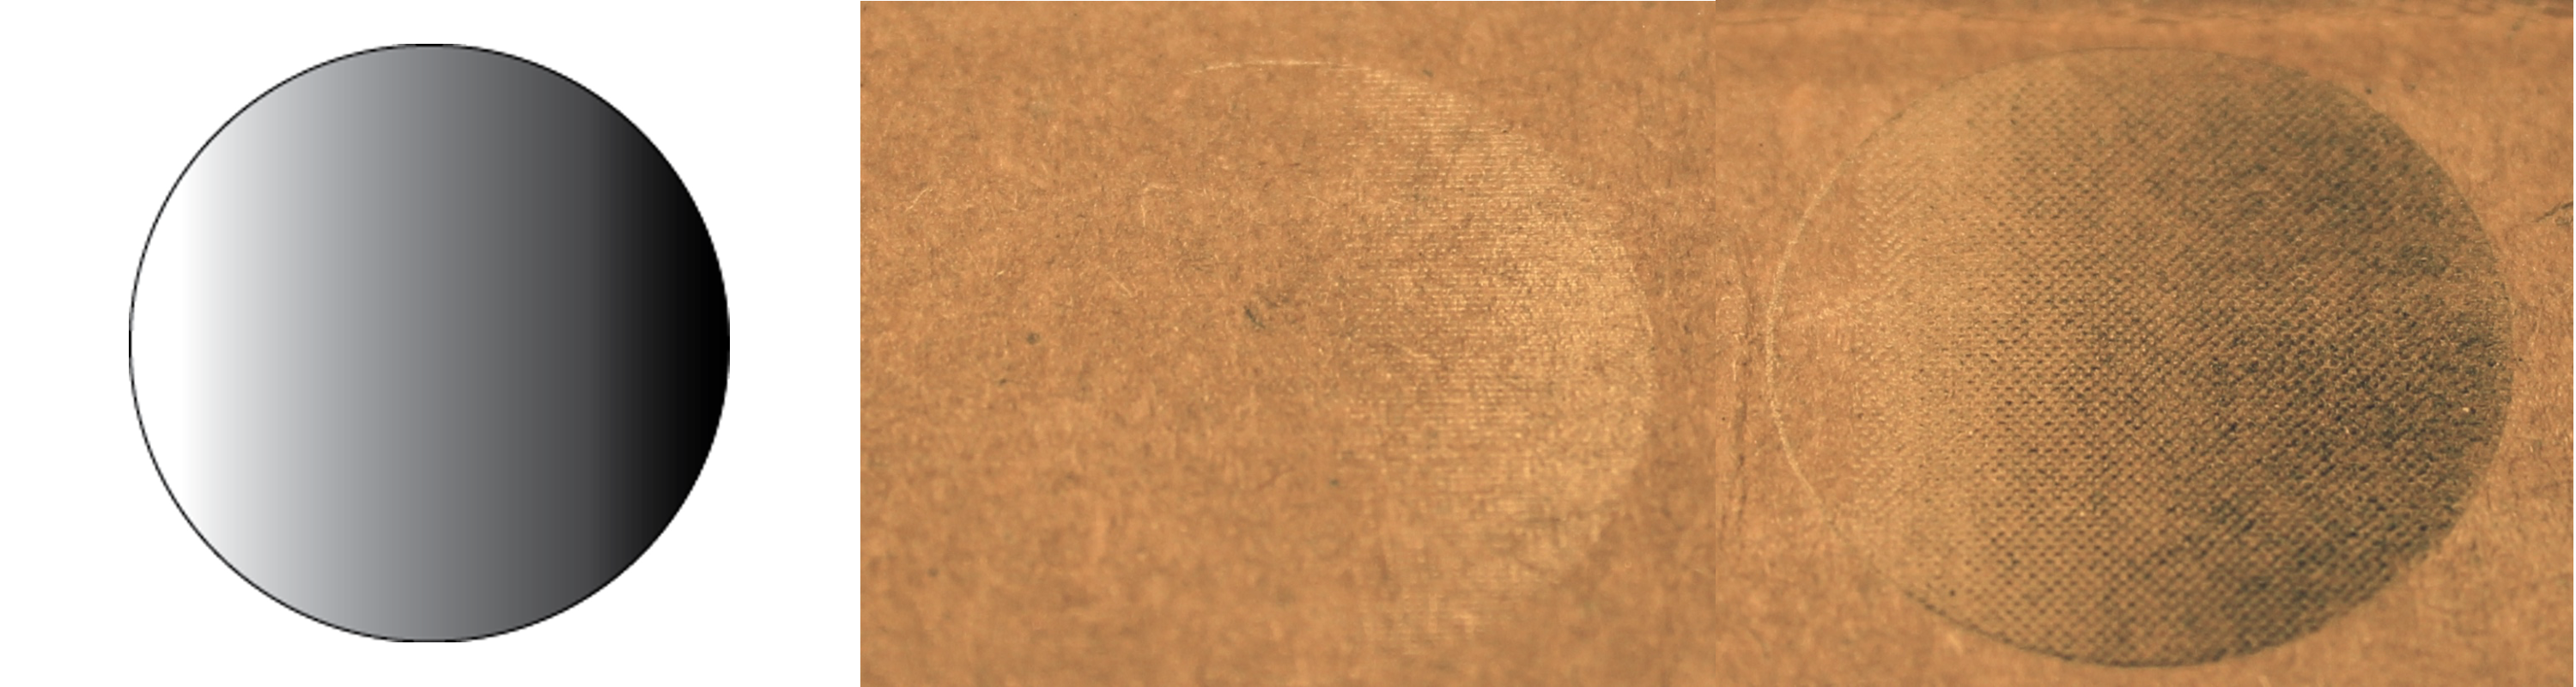
\includegraphics[width=0.4\textwidth]{figures/rasters}
  \caption{%
  A drawing `rastered' into cardboard.
  \emph{Left}: the original image given to the laser cutter.
  \emph{Center}: an etching that too faint to see due to low power.
  \emph{Right}: an etching scorched into the cardboard due to high power and low speed.
  A user of the laser cutter has to manipulate the laser's parameters to get the desired appearance.}
\label{fig:rasters}
\end{figure}

To understand the trade-offs of this method of mixed initiative parameter space exploration, I will run a usability study.
Participants will be asked to recover a configuration for rastering an image that matches an exemplar I provide.
The method of parameter exploration will be varied:
in one condition, participants explore configurations on their own.
In the other, participants explore the configuration space prompted by the examples provided by the active learning algorithm.
Among other metrics, I will measure the total number of configurations tested, and Likert scale and open-ended feedback on perceptions of the experience.

The usability study will use a Universal Laser Systems VLS3.50 machine.
I have received clearance to work with this equipment.
Given the limited time available for the hardware, the proposed usability study will likely include around 4--6 participants.
